\documentclass{article}
% \documentclass{scrreprt}
\usepackage{graphicx} % Required for inserting images
\usepackage[english, russian]{babel}
\usepackage{subcaption}

\title{MovieMatch}
\author{Антонина Климчук}
\date{}

\begin{document}

\maketitle


\section{Введение}

\subsection{Цель проекта}
Цель: создать telegram-бота, который поможет компании людей выбрать фильм на вечер так, чтобы всех устроил

\subsection{Целевая аудитория}
\begin{enumerate}
    \item Любая компания, которая не всегда может найти фильм для просмотра всем вместе
    \item Человек, у которого закончились идеи о том, что бы посмотреть
\end{enumerate}


\subsection{Глоссарий}
\begin{itemize}
    \item \textbf{Игра} - раунд проведения выбора фильма для компании
    \item \textbf{Игрок} - пользователь, который в процессе игры
    \item \textbf{Начальный игрок} - игрок, который начал игру
    \item \textbf{Понравившийся фильм/сериал} - фильм/сериал, который пользователь в одной из игр отметил, как тот, который хочет посмотреть
    \item \textbf{Фильтр} - установление начальным игроком жанра, годов выпуска

\end{itemize}
\newpage

\section{Общее описание продукта}

\subsection{Структура проекта}

\begin{figure}[htbp]
  \centering
      \centering
      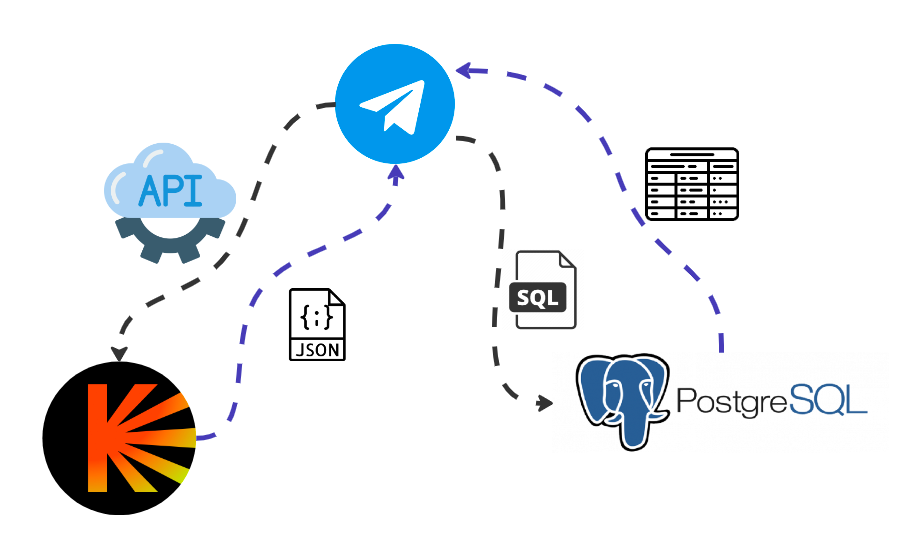
\includegraphics[width=1\textwidth]{project_structure.png}
      \label{fig:project diogram}
      \caption{Диаграма взаимодействия системы. На ней стрелочками показано от кого к кому с каким типом данных присылается запрос или ответ, запрос отмечается черной стрелочкой, ответ - синей}
  \label{fig:project structure}
\end{figure}



\begin{enumerate}
    \item Бот отправляет API запрос к кинопоиску с фильтрами, чтобы тот достал фильмы/сериалы
    \item Кинопоиск возвращает ему json с результатами
    \item Бот предлагает пользователям полученные фильмы
    \item Для каждого игрока бот запоминает понравившиеся фильмы и кладет их в базу данных
    \item По запросу пользователя бот достает понравившиеся фильмы игрока
\end{enumerate}

\subsection{Классы и характеристики пользователей}

Все пользователи относятся с одному классу - люди, которые не знают что хотят посмотреть и для них проблематично запомнить какой фильм/сериал когда-то заинтересовал.

\subsection{Операционная среда}
Для разработки телеграм бота используется PyCharm, Visual Studio Code на языке Python.

\subsection{Ограничения при проектировании}
Языком разработки телеграм бота является язык программированися Python, в качестве базы данных используется база данных PostgreSQL. Обмен данными между ботом и кинопоиском происходит через API. Для обмена данными между базой данных и телеграм ботом используется язык запросов SQL. 

\subsection{Документация пользователя}
\begin{itemize}
    \item Функция \textbf{/start} - начать общение с ботом, он присылает ознакомительное сообщение с описанием доступных команд.
\item Функция \textbf{/help} - получить список команд с описанием.
\item Функция \textbf{/start\textunderscore game} - начать игру в текущем чате.
\item Функция \textbf{/get\textunderscore list \textunderscore of \textunderscore liked} - 
олучить свой список понравившихся фильмов и сериалов.

\end{itemize}

\section{Системные функции}

\subsection{Функция принятия данных от пользователя}

Входными данными является текстовый запрос пользователя с помощью вызова нужной функции из представленных в /help. В обработке пользовательского запроса бот вызывает нужную функцию для ее обработки. Выходными данными так же являются текстовые данные.

\subsection{Функция обращения к кинопоиску}
Входными данными являются 'фильтр' из запроса пользователя с помозью которого и будет отправлятся запрос к кинопосику. Вызывает запрос GET с нужными параметрами из "фильтра". Выходными данными является json.

\subsection{Функция доставки данных в базу данных}
Входными данными является id пользователя и информация о фильме, которую надо положить в базу данных. Производится SQL запрос INSERT к базе данных с values id и информацией о фильме.

\subsection{Функция достать данные из базы данных}
Входными данными является id пользователя, для которого надо достать данные. Производится SQL запрос SELECT к базе данных с фильтром на id пользователя. Выходными данными явзяется выборка из базы данных.

\subsection{Функция обработки "понравившихся фильмов"}
Входными данными является id фильма, а так же текущий фильм. Вызывается функция доставки данных в базу данных.

\section{Нефункциональные требования}

\subsection{Раширяемость} 

    Проект должен поддерживать несколько обращений, например, проводить несколько "игр" одновременно в разных чатах.
\subsection{Интерфейс}
    Проект должен обладать понятным интерйфейсом, то есть наличие списка команд с объяснением их смысла, а так же читабельное, удобное представления информации о фильме во время "игры".
    
        

\section{Тестирование}

\subsection{Тестирование раширяемости}
Тестирование данного требования производится потем запуска нескольких обращений от пользователей из разных чатов.

\subsection{Тестирование корректного распознавания "понравившихся фильмов"}

Тестирование данной функции производится путем проверки наличия в базе даннх информации о фильме для нужного пользователя.
\end{document}

